\section{直言三段论的15个有效形式}

\begin{logicbox}[title=引言]
在标准式直言三段论的256种可能形式中,只有15种是有效的。本节将介绍这些有效形式及其古典命名系统,帮助我们快速识别有效三段论并应用于实际推理中。掌握这些形式,是理解亚里士多德式推理系统的关键。
\end{logicbox}

\begin{theorembox}[title=三段论的式与格]
\logicemph{式的定义}:三段论的\logicterm{式}取决于其中所含三个命题的类型(A、E、I、O)。

\logicwarn{式的数量}:直言三段论有64个不同的式,即这三个命题的64种可能组合:AAA、AAI、AAE等等,一直到EOO、OOO。

\logicemph{格的定义}:三段论的\logicterm{格}是其逻辑形状,由中项在前提中的不同位置决定。

\logicwarn{格的数量}:一共有四种不同的格,如果头脑中有一个图表或者用图标说明,就可以很清晰地记住这几个格,见图6—11:
\end{theorembox}

\begin{center}
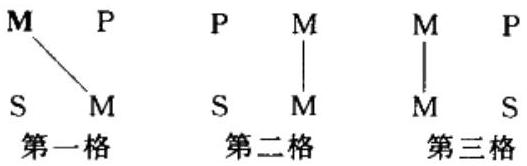
\includegraphics[width=\textwidth]{images/2025_05_15_6a28331d5e7c993ad07ag-288.jpg}

图6-11 三段论的四种格
\end{center}

\begin{center}
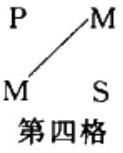
\includegraphics[width=\textwidth]{images/2025_05_15_6a28331d5e7c993ad07ag-288(1).jpg}
\end{center}

\logicwarn{四种格的特征}:从图中可见:

\begin{itemize}
  \item \logicterm{第一格}:中项是大前提的主项、小前提的谓项
  \item \logicterm{第二格}:中项在两个前提中都做谓项
  \item \logicterm{第三格}:中项在两个前提中都做主项
  \item \logicterm{第四格}:中项是大前提的谓项、小前提的主项
\end{itemize}

\logicemph{形式的计算}:64个式都可以有四个格。把两者结合起来,给定了三段论的式与格,也就唯一地确定了三段论的形式。因此,标准式直言三段论恰有$256(64 \times 4)$个可能的形式。

\logicwarn{有效性筛选}:这些形式中绝大部分是无效的。根据前一节阐明的三段论规则,我们可以排除那些违反了一条或几条规则的形式,剩下的就是直言三段论的有效式。256个形式中,只有15个形式不能被排除,因而它们是有效的。\cite{patzig1968}

\begin{theorembox}[title=古典命名系统的设计原理]
\logicemph{命名目的}:为更好地掌握三段论,古典逻辑学家给每一个有效式都起了独特的名称,每一个都完全刻画了其格与式。

\logicwarn{实用价值}:了解有效式的这个小集合,记住每一个有效形式的名称,对于我们实际运用三段论论证是很有帮助的。

\logicterm{设计原理}:
\begin{itemize}
  \item 这些名称都是精心设计的,每个名称都包含了三个元音
  \item 代表着被命名三段论的式(依据标准的顺序:大前提、小前提、结论)
  \item 对于同式不同格的有效三段论形式,都分别给它们指派唯一的名称
\end{itemize}

\logicemph{具体例子}:对于式为EAE的三段论,如果是第一格的就叫做Celarent,而如果是第二格的就叫做Cesare。\cite{lukasiewicz1957}
\end{theorembox}

\begin{examplebox}[title=命名系统的实用功能]
\logicwarn{识别功能}:这些名称曾经有(现在仍然有)很实用的功能:如果懂得只有式与格的某些特定组合是有效的,并且通过名字就能识别那些有效论证,那么,无论给出任何式或格的三段论,就都能立即判定其正误。

\logicemph{具体应用}:例如,AOO式只在第二格才是有效的。这个唯一的形式(AOO-2)就叫做Baroko。\cite{copi1980}

\logicterm{推理能力}:熟悉Baroko并能很容易指认它的人就会确信这个式的其他格都是无效的,是必须拒斥的。

\logicwarn{学习价值}:
\begin{itemize}
  \item 快速识别有效与无效论证
  \item 提高逻辑分析的效率
  \item 增强论证评估的准确性
  \item 培养严谨的逻辑思维
\end{itemize}
\end{examplebox}

\begin{logicbox}[title=三段论理论的历史意义与实用价值]
\logicemph{古典研究}:古典逻辑学家很细致地研究了这些形式,谙熟它们的结构和逻辑"感应"。

\logicwarn{系统功能}:这种精心设计好的逻辑系统,会使得一个人在言语或文本中碰到三段论论证时,能立即确切指认哪些是有效的,哪些是无效的。

\logicterm{传统训练}:许多世纪以来,逻辑训练的一种常用方式,就是通过给出三段论有效形式的名称,来为三段论论证的可靠性进行辩护。

\logicemph{学养标志}:而在激烈的日常论辩中具备这种迅速识别有效论证与无效论证的能力,一直被视为富有学养、思维敏锐的标志。

\logicwarn{论证力量}:而依赖演绎论证所建立起来的论证链条之坚固也得到了充分显示。一旦完全掌握三段论理论,这种实际论辩能力就会得到富有成效的令人愉悦的提升。

\logicterm{亚里士多德的贡献}:三段论论证曾经有如此广泛的应用,并被普遍视为学术论证最不可缺少的工具,因此,最先系统论述三段论理论的学术大师亚里士多德,得到了人们上千年的尊崇。他关于三段论的分析的论集迄今仍沿用着一个简单但令人肃然起敬的名字:Organon,即《工具论》。
\end{logicbox}

\logicwarn{学习建议}:作为这个著名逻辑体系的初学者,我们对三段论的掌握可能难以非常精通。但列出所有有效三段论形式并加以熟练掌握,无疑是最为有用的。

\logicemph{分组规律}:15个有效三段论形式(布尔解释下的)可以根据格的不同分为四组:在前三个格中都有四个有效形式,第四格有三个有效形式。\cite{patzig1968}

\logicterm{完整列表}:下图即列出了15个有效形式,以及它们相应的传统名称:

\begin{theorembox}[title=标准式直言三段论的15个有效形式]
\logicemph{第一格}(中项在大前提中做主项、在小前提中做谓项):
\begin{itemize}
\item 1. \logicterm{AAA-1 Barbara}
\item 2. \logicterm{EAE-1 Celarent}
\item 3. \logicterm{AII-1 Darii}
\item 4. \logicterm{EIO-1 Ferio}
\end{itemize}

\logicwarn{第二格}(中项在两个前提中都做谓项):
\begin{itemize}
\item 5. \logicterm{AEE-2 Camestres}
\item 6. \logicterm{EAE-2 Cesare}
\item 7. \logicterm{AOO-2 Baroko}
\item 8. \logicterm{EIO-2 Festino}
\end{itemize}

\logicemph{第三格}(中项在两个前提中都做主项):
\begin{itemize}
\item 9. \logicterm{AII-3 Datisi}
\item 10. \logicterm{IAI-3 Disamis}
\item 11. \logicterm{EIO-3 Ferison}
\item 12. \logicterm{OAO-3 Bokardo}
\end{itemize}

\logicwarn{第四格}(中项在大前提中做谓项、在小前提中做主项):
\begin{itemize}
\item 13. \logicterm{AEE-4 Camenes}
\item 14. \logicterm{IAI-4 Dimaris}
\item 15. \logicterm{EIO-4 Fresison}
\end{itemize}
\end{theorembox}

\footnotetext{(8)在传统或者亚里士多德式解释下,有效式的数目是19个或者24个,因为其中已包含了布尔解释下并不有效的弱化(weakened)格式——后者的结论比前提断定得更少。}
\footnotetext{(9)传统名称中所包含的元音是由拉丁语创造出来的一种记忆方法,其含义在拉丁语中是完备的;不过,无论说什么语言的人,都能通过观察名称中包含的元音,看出该三段论属于哪个式。}
\footnotetext{(10)传统的有记忆价值的名称是Baroco而不是Baroko;但在汉语中,似乎很难将c和k的发音分得很开,所以这里保持拼写一致用k取代c。}
\footnotetext{(11)第四格下有效三段论较少,是因为这种格式的三段论总是有点绕弯子,因而不太直接,似乎是人工制造的而不是自然思维的产物——但这也不影响其有效性。}

\begin{center}
\fbox{\parbox{0.95\textwidth}{
\textbf{本节要点}
\begin{itemize}
\item 标准式直言三段论共有\textbf{256种可能形式}(64个式 × 4个格)
\item 其中只有\textbf{15个有效形式}(布尔解释下)
\item \textbf{古典命名系统}:每个有效形式都有特定名称
  \begin{itemize}
  \item 名称中的三个元音对应三段论的式(大前提、小前提、结论)
  \item 例如:Barbara (AAA-1)、Celarent (EAE-1)、Baroko (AOO-2)
  \end{itemize}
\item \textbf{格的分布}:
  \begin{itemize}
  \item 第一格:4个有效形式
  \item 第二格:4个有效形式
  \item 第三格:4个有效形式
  \item 第四格:3个有效形式
  \end{itemize}
\item 掌握这些有效形式及其名称,有助于快速识别有效论证和无效论证
\end{itemize}
}}
\end{center}